\begin{surferPage}[六次曲线(30 尖点)]{巴斯带30尖点的六次曲线}
在沃尔夫巴斯构造了具有最多奇异点(65个)的六次曲面之后,他的两个学生也构造了创世界纪录的更高次数的曲面。巴斯开始考虑对给定的次数的曲面可以构造最多个尖点的问题。
他的具有65个 $A_1^{+-}$型(双锥型)奇异点的六次曲面可以用来构造尖点。这便产生了30个\[P_6 - \alpha \cdot K^3=0.\]其中$P_6$是正二十面体中与构造巴斯六次曲面时相同的一个对称面,$K$同样是单位球面。

    \vspace*{-0.4em}
    \begin{center}
      \begin{tabular}{c@{\ }c@{\ }c@{\ }c}
        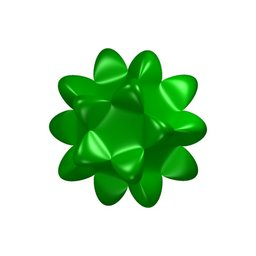
\includegraphics[height=1.2cm]{./../../common/images/barthsextic_30A2}
        &
        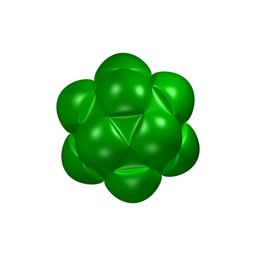
\includegraphics[height=1.2cm]{./../../common/images/barthsextic_30A2_3}
        &
        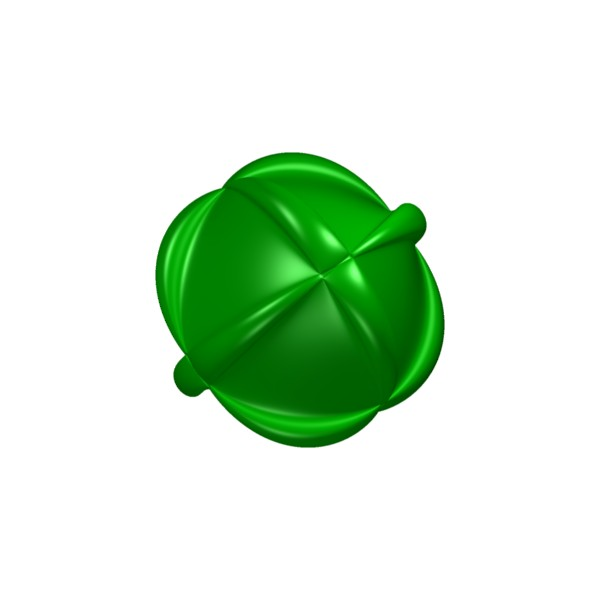
\includegraphics[height=1.2cm]{./../../common/images/barthsextic_30A2_5}
        &
        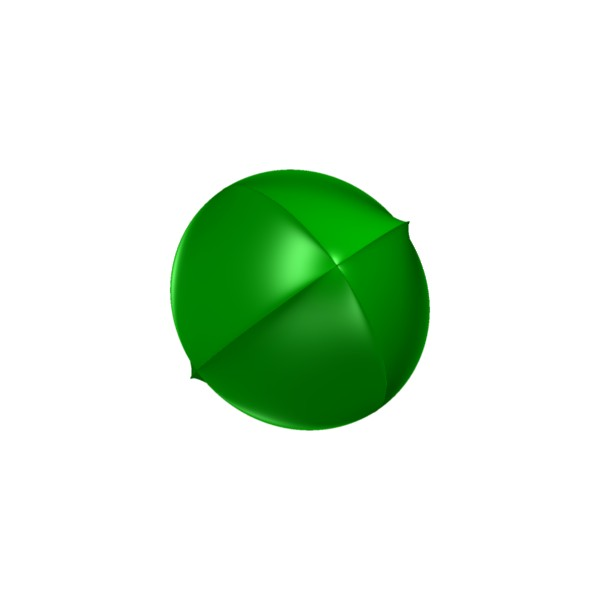
\includegraphics[height=1.2cm]{./../../common/images/barthsextic_30A2_6}
      \end{tabular}
    \end{center}    
    \vspace*{-0.3em}

这是六次曲面上实尖点数当今世界纪录最多的一个例子,它的复尖点个数是36。
\end{surferPage}
